\chapter{Background} \label{bkgnd}

\section{Limb Imaging \& The Atmosphere}
Discussion about general limb imaging, background, history.

\subsection{UTLS Overview}
Background of the UTLS region and the species that should be measured.

\subsection{Techniques}
Three techniques for limb imaging involve limb emission, limb scattering, and solar occultation. Limb emission works by measuring radiation emitted by the atmosphere, either thermally or photochemically, along the instrument line of sight (LOS). These are generally low signal level but can be measured with sensitive instruments. Limb scattering instruments measure photons originating from the sun that have been scattered from the atmosphere.   Solar occultation measurements look through the atmosphere directly at the sun and measure the spectral attenuation of the solar irradiance. Note that occultation can also been done with the moon or stars as the source.

\subsection{Instruments}
Briefly talk about various instruments before going into a bit more detail below about MIPAS and GLORIA

\subsubsection{MIPAS}
A key early instrument to measure limb emission from space is the Michelson Interferometer for Passive Atmospheric Sounding (MIPAS)~\cite{MIPAS_instrument}. MIPAS used limb emission to measure atmospheric spectral radiances in the spectral ranges of 685-970 cm\textsuperscript{-1}, 1020-1170 cm\textsuperscript{-1}, 1215-1500 cm\textsuperscript{-1}, 1570-750 cm\textsuperscript{-1}, and 1820-2410 cm\textsuperscript{-1}, which provided data on temperature, trace species and cloud distributions. The core of the instrument is a Fourier Transform Spectrometer (FTS) that could detect mid-infrared emissions. The goal of this instrument was to observe global changes in the composition of the atmosphere resulting from pollution and other man-made effects. It provided profiles of H\textsubscript{2}O, O\textsubscript{3}, CH\textsubscript{4}, N\textsubscript{2}O, HNO\textsubscript{3}, and NO\textsubscript{2} during its operation as part of the Environmental Satellite (EnviSat), a European Space Agency satellite~\cite{MIPAS_instrument}.

MIPAS, and similar instruments such as the Atmospheric Chemistry Experiment Fourier Transform Spectrometer (ACE-FTS), utilized Fourier transform spectrometers in their measurements~\cite{SPARC}~\cite{ACE_conference}. However, a limitation of these instruments is that they are not imaging instruments; they have only a single detector pixel. Limb scanning must be used to cover the atmospheric limb, where the instrument moves the line of sight upwards and downwards. However, new and larger data storage and transfer techniques have led to the usage of the imaging Fourier Transform Spectrometer (IFTS), which generates a high amount of data. With a larger throughput, more pixels can be used to create a much wider FOV that covers the atmospheric limb, thus not needing any movement of the instrument. The first instrument to demonstrate the imaging FTS concept for atmospheric measurements is a second generation MIPAS instrument, the Gimballed Limb Observer for Radiance Imaging in the Atmosphere (GLORIA) instrument~\cite{GLORIA_concept}.

\subsubsection{GLORIA}
GLORIA is an airborne limb imaging instrument operating in the thermal infrared region from 780 cm\textsuperscript{-1} to 1400 cm\textsuperscript{-1} and is conceptually like the LIFE instrument that is the focus of this thesis. GLORIA consists of an IFTS device mounted on a gimbal and provides high spatial and spectral resolution measurements of the upper troposphere/lower stratosphere (UTLS)~\cite{GLORIA_concept}~\cite{GLORIA_PhD}. GLORIA utilizes a two-dimensional pixel array to obtain this high spatial resolution, as no spatial scanning of the imager is necessary. The detector is sensitive to numerous species, including H\textsubscript{2}O, O\textsubscript{3}, CCl\textsubscript{4}, HNO\textsubscript{3}, ClONO\textsubscript{2}, HO\textsubscript{2}NO\textsubscript{2}, and CFCs. With the high spatial resolution, GLORIA will measure the steep gradients in trace gases and characteristics of clouds in the UTLS region, as well as provide insight into the stratospheric-troposphere-exchange that has been affected by climate change~\cite{GLORIA_PhD}~\cite{GLORIA_objectives}.

\subsubsection{LIFE}
The LIFE instrument prototype is being developed at the University of Saskatchewan and is designed to build on the success of GLORIA.  A collaboration between the University of Saskatchewan, Canadian Space Agency (CSA), Environment and Climate Change Canada (ECCC) and ABB, it is designed to take high vertical resolution measurements of atmospheric thermal emission over the 7-14 \textmu m spectral range to retrieve key radiative species in the UTLS including H\textsubscript{2}O, HNO\textsubscript{3}, O\textsubscript{3}, N\textsubscript{2}O, and CH\textsubscript{4}. Similar to GLORIA, the goal of LIFE is to fill the gap in information in the UTLS region. LIFE is designed to meet or exceed the capabilities of GLORIA and aims to shrink the complexity of an IFTS atmospheric sensing instrument. The LIFE instrument utilizes a 16-pixel linear array detector to image through an IFTS, to obtain a high vertical resolution of these key species. The instrument was first tested on a high-altitude balloon flight on August 31-September 1, 2019.

\section{Thermal Design}
Talk about the basics of thermal design at an atmospheric instrument level and the environment. Can perhaps briefly mention self-emission.

\subsection{Thermal Phenomena}
Overview of the phenomena at altitudes:

\subsubsection{Radiation}
Radiation heat transfer occurs through electromagnetic radiation, where a body emits energy. Radiation can often be neglected, but in a vacuum and at higher temperatures it plays an important role. The flux of energy radiation from a body in W/m\textsuperscript{2}, \textit{q}, can be described by the Stefan-Boltzmann law, in Equation \ref{SB_law}.

\begin{equation} \label{SB_law}
    q(T) = \epsilon \sigma T^{4}A
\end{equation}

where the Stefan-Boltzmann constant, \textsigma, is 5.670374 × 108 W/m\textsuperscript{2}K\textsuperscript{4}, {\textepsilon} is the emissivity of the surface, \textit{A} is the area of the surface, and \textit{T} is the absolute temperature. This formula can be altered for an object radiating to its surroundings, shown in Equation \ref{SB_surroundings}.

\begin{equation} \label{SB_surroundings}
    q(T) = \epsilon \sigma (T_h^4-T_c^4)A_h
\end{equation}

where T\textsubscript{h} is the temperature of the hot body, T\textsubscript{c} is the temperature of the cold blackbody, and A\textsubscript{h} is the surface area of the hot body~\cite{heat_transfer_textbook}~\cite{FEA_SW}. When dealing with thermal design in a vacuum, the surface area and emissivity are two variables that can be controlled and help to either dissipate or maintain heat.

\subsubsection{Conduction}
Conduction heat transfer takes place within bodies by diffusion of energy and is an important part of all thermal design. The heat flux through the body in W/m\textsuperscript{2}, \textit{q}, is described by Fourier’s Conduction Law, shown in Equation \ref{FC_law}.

\begin{equation} \label{FC_law}
    q(T) = -k\nabla T
\end{equation}

Here \textit{k} is the thermal conductivity of the material and $\nabla$\textit{T} is the temperature gradient. For an anisotropic material, the conductivity is a tensor and the temperature gradient forms a vector. The thermal conductivity is dependent on the material and has units of W/mK~\cite{heat_transfer_textbook}~\cite{FEA_SW}. The design control for the conduction of heat relies on \textit{k}, thus the material chosen.

\subsubsection{Convection}
[TODO]

\subsection{Balloon Environment}
Thermal design in an important part of both space and atmospheric instruments. Through the ascent phase of a high-altitude balloon flight, the instrument will reach such extreme temperatures as -80°C. On the ground, most instruments are cooled with a combination of conduction and convection. Convection often plays a large role by using fans to cool the instrument. However, at high altitudes, with convection no longer available due to the lack of air (or any surrounding fluid), all thermal heating and cooling must be done with radiation and conduction. 
 % These are taken from two different sections of the advisory report so make sure its cleaned up to flow nicely.
 Temperatures the instrument will endure during the float period of the flight can be found from previous flight data of similar instrumentation. The temperature data from the balloon gondola during a 2018 flight from Timmins, Ontario, was measured by the National Centre for Space Studies (CNES), who operated the balloon. Temperature was also measured for one of the instruments on-board, the Canadian Atmospheric Tomography System (CATS) instrument. These two sets of temperatures can be used to provide an example of what the LIFE instrument will experience during flight. The temperature data from the 2018 flight is shown in Figure \ref{fig:2018_timmins_temps}~\cite{CATS_report}. 
 
 \begin{figure}[h]
\centering
  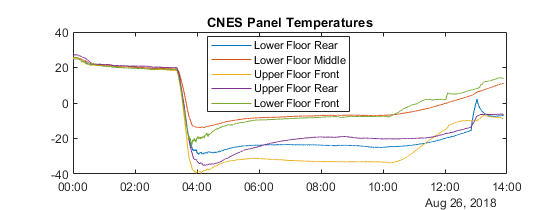
\includegraphics{chap2_images/CNES_temps_CATS_2018.png}
  \caption{High altitude balloon temperatures during 2018 flight in Timmins, Ontario}
  \label{fig:2018_timmins_temps}
\end{figure}

It can be seen in Figure \ref{fig:2018_timmins_temps} that the lowest gondola temperature reached during the flight was -40°C, which occurs when travelling through the cold tropopause. This was used as the worst-case scenario temperature for the thermal simulations done within the thesis work. The upper temperature for thermal modelling was set at 20°C, the temperature of the lab. For most of the flight the baseplate that the instrument will sit on is approximately -30°C, based on the worst-case gondola floor temperature from Figure \ref{fig:2018_timmins_temps}. 

Atmospheric instruments often have delicate optics or electronics, so the thermal characteristics of the instrument are a very important part of the design. Particularly for thermal imaging instruments, the optics must be carefully controlled in order to reduce the thermal radiation background, or self-emission, effect on measurements. Self-emission can lead to systematic error in the data, as part of the data collected are thermal properties from the optics rather than the atmosphere. Various instruments use different methods to maintain appropriate operational conditions for the instrument. The MIPAS and GLORIA thermal designs are discussed here for context. 

\subsection{Self-Emission}
Discuss self-emission at a deep background level, similar to what Jeff and I talked about and what Ethan has been looking into. Don't discuss the design of LIFE at all that allowed us to ignore this more than most instruments.

[TODO]

\subsection{Instruments} \label{GLORIA_MIPAS_thermal}
Summarize thermal designs of previous instruments. Part of this is described above in the balloon environment opening.

\subsubsection{MIPAS}
The MIPAS instrument used an FTS for the detection of limb emission spectra. To avoid self-emission from the FTS, it was cooled and maintained at 210K. The optics and detector of MIPAS were also actively cooled and kept below 70K to reduce both thermal emission and internal noise contribution. Cooling for components required the use of multiple Stirling coolers and good thermal insulation. All optics were fully thermally isolated from the rest of the instrument which led to a complex optical design~\cite{MIPAS_instrument}.

\subsubsection{GLORIA}
The GLORIA instrument similarly uses a cooled FTS system. The desired operating range of the lens and FTS system is 200-220K, to again self-emission and resulting noise. To maintain this low temperature while operating on an aircraft, a complex system was designed that uses liquid carbon dioxide. This CO\textsubscript{2} is sprayed into a cooler tank under high pressure through small injection pipes, which sharply drops the pressure at the exit. This leads to adiabatic cooling and the generation of CO\textsubscript{2} snow, which keeps the instrument operating at the required temperature for 24 hours. Liquid nitrogen is also a cooling option but this could not be used during flight due to safety and weight constraints and is only used in the lab. To avoid data contamination due to the CO\textsubscript{2}, the FTS is sealed. Around this entire closed system vacuum insulation panels are used. Finally, the detector itself must be cooled to a temperature of 50K, which was accomplished with a Stirling cooler~\cite{GLORIA_concept}~\cite{GLORIA_thermalmech}
% There is a paragraph following this in the advisory report that goes into the LIFE thermal considerations at a similar level. There is not really a good place to put it in this thesis but can be used if necessary.

\section{IR Detectors}
Talk about different types of IR Detectors

\subsection{MCT Detectors}
The detector chosen for use in the LIFE instrument is known as a Mercury Cadmium Telluride (MCT, or HgCdTe) detector. This semiconductor detects photons in the short-, mid-, and long-range infrared regime. Semiconductor characteristics that make this material preferable include long minority carrier lifetime, low carrier concentration, and small effective mass and high mobility~\cite{MCT_Detectors}. Other advantages of this detector include high response and sensitivity to infrared radiation. The GLORIA instrument uses a 2562-pixel MCT detector array~\cite{GLORIA_concept}. A drawback of the high sensitivity of these detectors is to lower noise as much as possible, they must be kept at very low temperatures. As described in Section \ref{GLORIA_MIPAS_thermal}, most detectors including those in GLORIA and LIFE are cooled to 70K or lower. The LIFE MCT detector setup is described in more detail in Chapter \ref{detector}.

\subsection{Non-linearity}
MCT detectors operate via either photovoltaic (PV) cells or photoconductive (PC) cells. PV detectors are used for shorter wavelength applications, whereas PC detectors, such as those used in LIFE, can be used for wavelengths up to 20\textmu m. Photoconductors exhibit a change in conductance when radiant power is applied, and the detector is operated with a constant bias current in order to sense the change in conductance, which is proportional to radiant flux. A voltage change is measured across the detector. An issue that arises is this voltage change across the detector is not linear with incident photon flux. This is due to a variety of reasons, but mainly due to the intrinsic non-linearity of semiconductors and their band gaps, as well as the non-linearity of the voltage as it approaches saturation~\cite{current_measurement_MCTs}~\cite{MCT_linearity}.  This non-linearity may be decreased through characterization of the detector, by changing the bias voltage and the current offset.

\subsection {Responsivity}
In addition to non-linearity, another characteristic of MCT detectors that can be determined and optimized is the responsivity. The detector responsivity is a measure of the sensitivity of the detector to incoming signal. Ideally, the higher the responsivity, the better the performance of the detector~\cite{GLORIA_PhD}. A basic circuit for measuring the responsivity is a circuit consisting of a bias battery supply \textit{V}, a load resistance \textit{R\textsubscript{L}}, and a detector with a dark current \textit{R\textsubscript{0}}. When radiation falls on the detector, the responsivity $\mathcal{R}_s$ given by Equation \ref{responsivity_eq_1}.

\begin{equation} \label{responsivity_eq_1}
    \mathcal{R}_s = \frac{V_s}{\phi h \nu A}
\end{equation}

Here $\phi$ represents the number of photos of frequency $\nu$ incident on detector \textit{A}. In the small signal approximation, the signal voltage \textit{V\textsubscript{s}} of this circuit is given by Equation .

\begin{equation}
    V_s = V \frac{R_L}{(R_L+R_0)^2}(-\Delta R_0)
\end{equation}

Here $\Delta R_0$ is the change in resistance of the detector due to illumination~\cite{MCT_responsivity}. The method of finding the responsivity in the case of LIFE is described in detail in Chapter \ref{detector}.